\chapter{Simulações}
\label{cap:III}
\section{Introdução}
 Neste capítulo mostrarei resoluções de algumas aproximações de funções e resolução de equações diferenciais utilizando métodos discutidos anteriormente. Todas as figuras obtidas aqui e implementação dos métodos foram feitas a partir da linguagem \emph{Julia}.

\section{Convergência do erro de interpolação utilizando o método espectral}
	Vamos agora ver a convergência do erro da aproximaçãode uma função de runge $\frac{1}{1+x^2},\ x\ \in [-5,5]$, para pontos \emph{equidistantes} e pontos igualmente espaçados, utilizando o polinômio de \textbf{Lagrange}.
	As aproximadas obtidas para raízes equidistantes e raízes de chebishev são:\\	
\begin{figure}[!ht]
  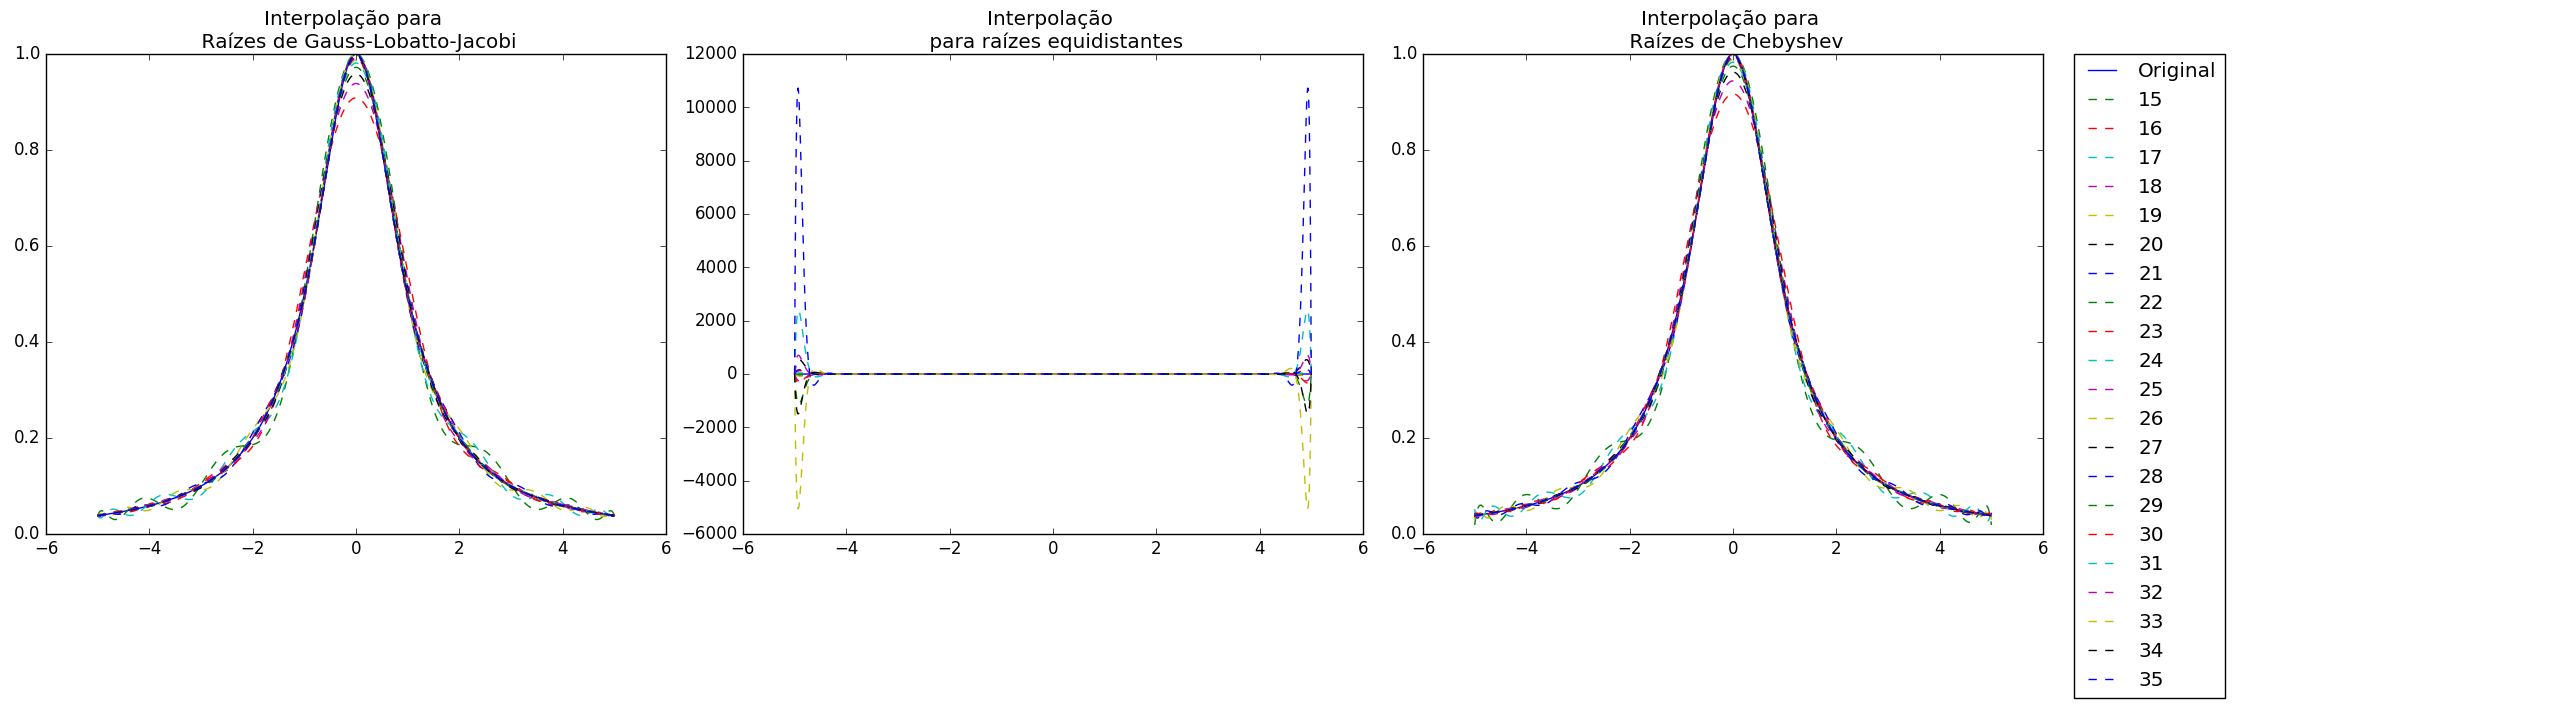
\includegraphics[width=0.8\textwidth,center]{figuras/interpolacao_todas.png}
  \caption{interpolação de polinômios de alta ordem com raízes de Gauss-Lobatto-Jacobi, igualmente espaçados, Chebyshev}
\end{figure}
Notamos novamente que para diferentes  polinômios de lagrange de alta ordem utilizando pontos igualmente espaçados, a aproximação nos pontos próximos das extremidades um erro  grande, enquanto que para pontos distribuídos usando as raízes de Chebyshev e de Gauss-Lobatto-Jacobi se comportam bem nessas regiões. Agora, iremos verificar a convergência desse erro, analizando o erro máximo para cada escolha de raízes.

\pagebreak
\begin{table}[h]
\centering
\caption{tabela de erros máximos para os diferentes tipos de raízes}
\label{my-label}
\begin{tabular}{|l|l|l|l|}
\hline
Grau & equidist & glj       & chebyshev     \\ \hline
15   & 7.19     & 4.925e-02 & 4.660e-02 \\
16   & 2.11     & 9.128e-02 & 8.309e-02 \\
17   & 14.39    & 3.480e-02 & 3.261e-02 \\
18   & 4.22     & 6.138e-02 & 5.590e-02 \\
19   & 29.19    & 2.417e-02 & 2.249e-02 \\
20   & 8.58     & 4.126e-02 & 3.758e-02 \\
\vdots   & \vdots              & \vdots    & \vdots    \\
30   & 333.94   & 5.651e-03 & 5.154e-03 \\
31   & 2384.73  & 2.229e-03 & 2.061e-03 \\
32   & 704.08   & 3.797e-03 & 3.463e-03 \\
33   & 5058.99  & 1.510e-03 & 1.402e-03 \\
34   & 1494.38  & 2.551e-03 & 2.328e-03 \\
35   & 10719.90 & 1.025e-03 & 9.488e-04 \\ \hline
\end{tabular}
\end{table}
Comparando as escolhas de raízes dos problemas conseguimos ver que a convergência do erro usando as raízes equidistantes aumenta conforme o grau do polinômio aumenta. Enquanto que para as raízes de Chebyshev e Gauss-Lobatto-Jacobi, os erros convergem algebricamente. 
\begin{figure}[!ht]
  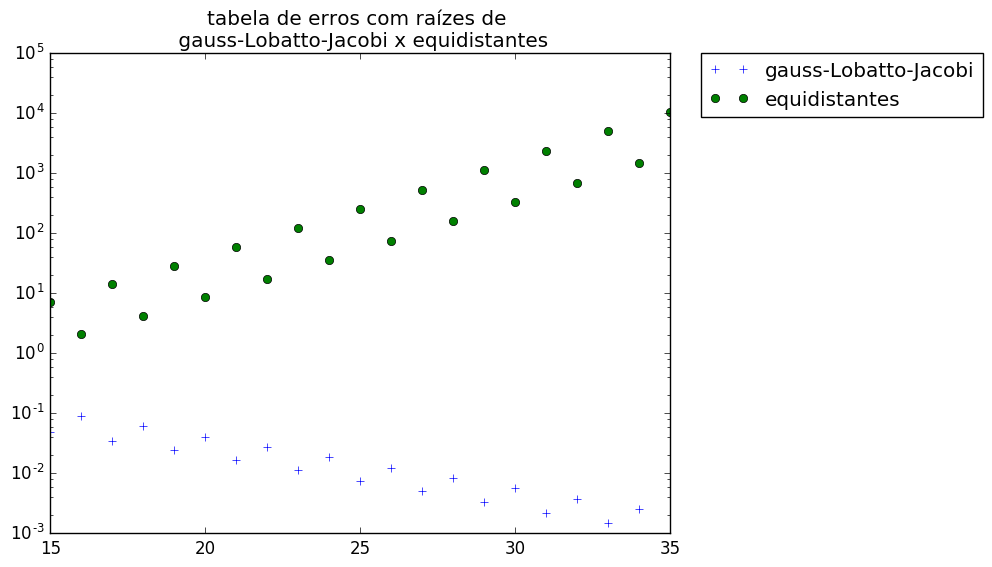
\includegraphics[width=0.5\textwidth,center]{figuras/glj_equi.png}
  \caption{comparação semilog  dos erros e graus de liberdade de raízes de glj versus equidistante }
\end{figure}
\begin{figure}[!hb]
  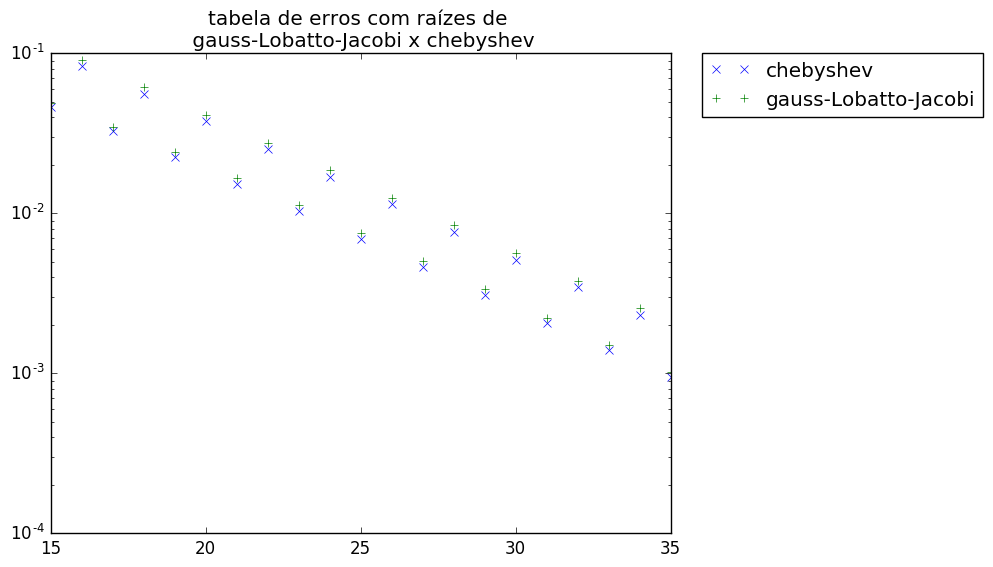
\includegraphics[width=0.5\textwidth,center]{figuras/glj_cheb.png}
  \caption{comparação semilog  dos erros e graus de liberdade de raízes de glj versus Chebyshev}
\end{figure}
\\
Notamos que embora a convergência, utilizando ambas as raízes dos polinômios, tenham o mesmo comportamento, podemos observar que como demonstrado  anteriormente a escolha do Polinômio de Chebyshev é o que melhor aproxima a função do fenômeno de Runge observando uma inclinação menor do erro.

\subsection{Convergência do erro de interpolação utilizando método H}
 Tendo aproximado a função de runge acima, utilizaremos um novo método chamado método H,método no qual subdividimos o problema em $n$ elementos de tamanho $H$. Iremos comparar o efeito desse método contra o método espectral anterior utilizando as mesmas raízes de aproximação, Gauss-Lobatto-Jacobi.
 
\begin{figure}[!ht]
  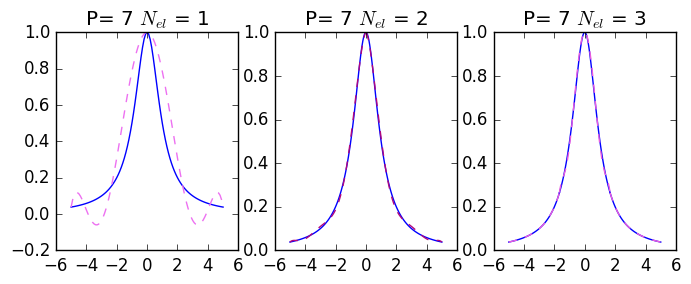
\includegraphics[width=0.8\textwidth,center]{figuras/interp_usando_FEM.png}
  \caption{gráficos das aproximações fixado o grau do polinômio em 7 e subdividimos o domínio em $N_{el}$ elementos }
\end{figure}
\begin{figure}[!hb]
  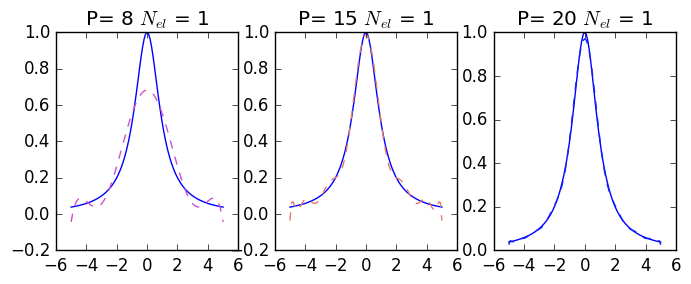
\includegraphics[width=0.8\textwidth,center]{figuras/interp_usando_FEMfixo.png}
  \caption{gráficos das aproximações fixado o número de elementos em 1 e utilizamos polinômios de grau elevado}
\end{figure}

\begin{figure}[!hb]
  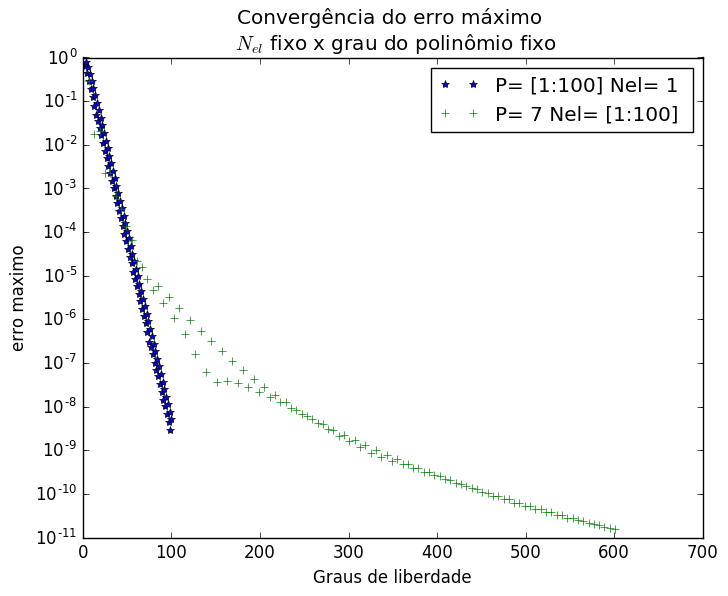
\includegraphics[width=0.7\textwidth,center]{figuras/convergencia_erro_FEM2.png}
  \caption{Convergência dos erros entre polinômios fixos e polinômios de grau elevado}
\end{figure}

 Notamos então no gráfico  que para o método utilizando o grau do polinômio fixo e variando o número de elementos, a convergência do erro é bem mais rápida que no caso onde variamos somente o grau do polinômio.
\section{Método HP na resolução de equações diferenciais}

 Agora, resolveremos uma equação diferencial de segundo grau. Para tanto, irei apresentar uma equação com solução conhecida ($sin(2\ k \pi x)$. Nesse caso, definirei o problema com a condição de fronteira de \emph{Dirichlet}, definindo assim o valor nas extremidades do domínio. Abaixo, está um comparativo entre a solução exata e a solução aproximada do problema utiliz
\begin{align}
y'' + y &= (1 + 4 (k \pi)^2)sin(2 k \pi x) \\
y(-1) &= sin(-2\ k \ \pi ) = 0 ,\ y(1) = sin(2\ k\ \pi) = 0 \ \ \forall k = 1,2,\dots \\
\end{align}	
\begin{figure}[!h]
  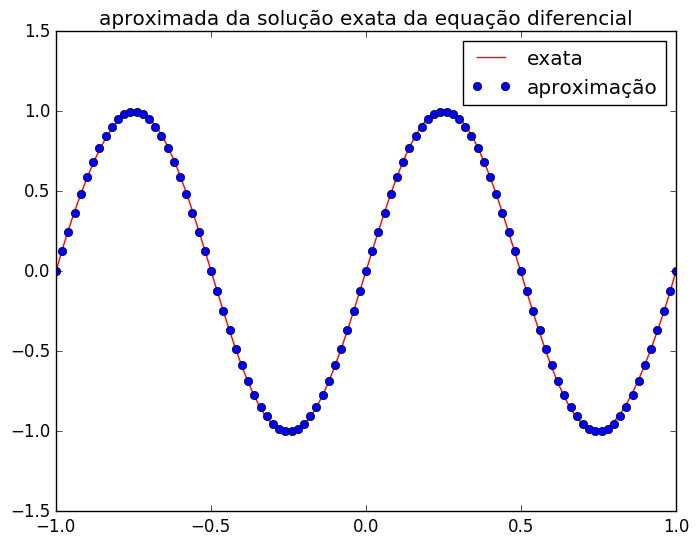
\includegraphics[width=1\textwidth,center]{figuras/solu_edo_simul.png}
  \caption{comparação entre a solução exata e a aproximada usando P= 10 e $N_{el} = 10$ }
\end{figure}
 Abaixo observaremos a variância do erro máximo para dois casos do Método \emph{HP}. No primeiro fixamos o grau P do polinômio interpolador e variamos o tamanho \emph{H} dos elementos, assim variando o número de elementos que discretizamos o problema. No segundo, é o inverso disso, em que fixamos o número de elementos e variamos o grau do polinômio interpolador P.


\begin{figure}[!hb]
  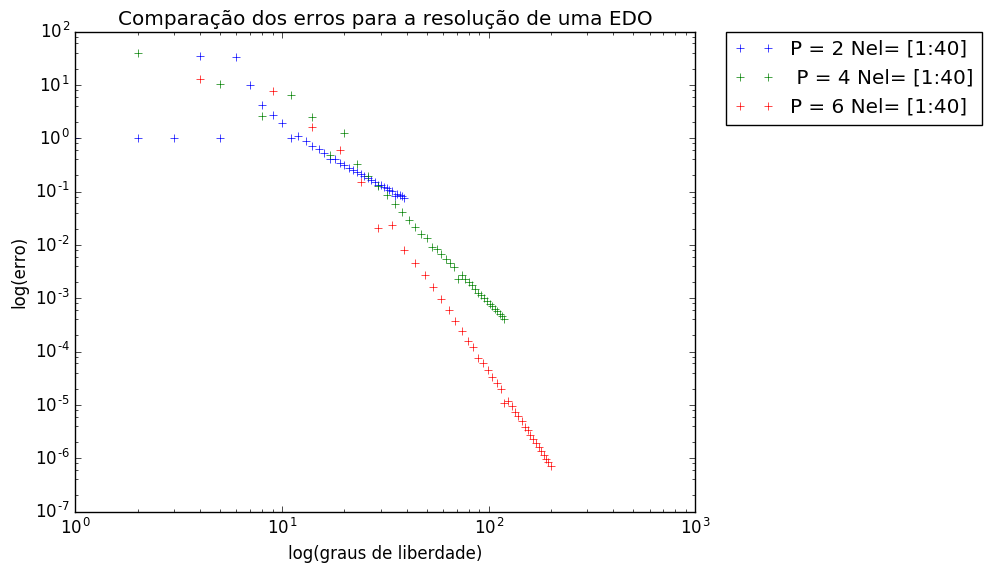
\includegraphics[width=1\textwidth,center]{figuras/convergencia_erro_EDO_h.png}
  \caption{convergência do log(erro) em função dos log(graus de liberdade) fixando o grau do polinômio em P e variando o número de elementos entre 1 a 40 }
\end{figure}


\begin{figure}[!hb]
  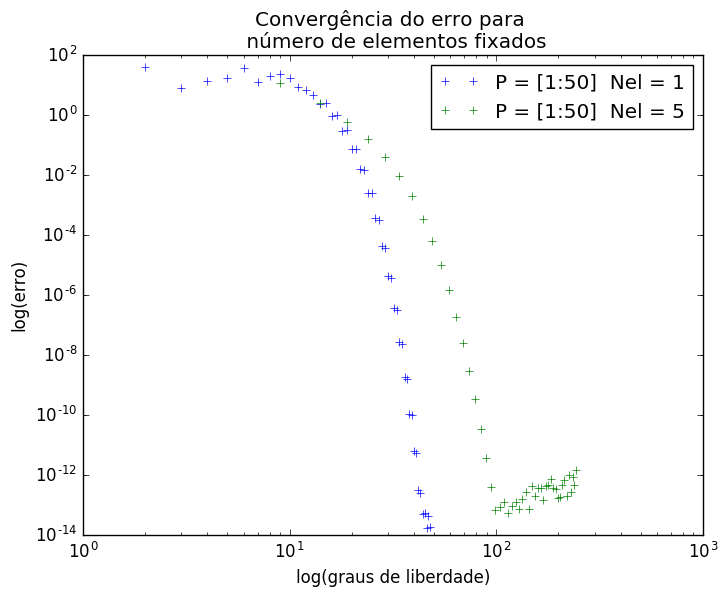
\includegraphics[width=1\textwidth,center]{figuras/convergencia_erro_EDO_p.png}
  \caption{convergência do log(erro) em função dos log(graus de liberdade) fixando o número de elementos e variando grau do polinômio em P  }
\end{figure}

\subsection{Condição de Neumann}



